% All figures describe one training seed and the same 24 development scenes.
% Intervals, where reported separately, do not measure across-seed uncertainty.
\begin{figure*}[t]
\centering
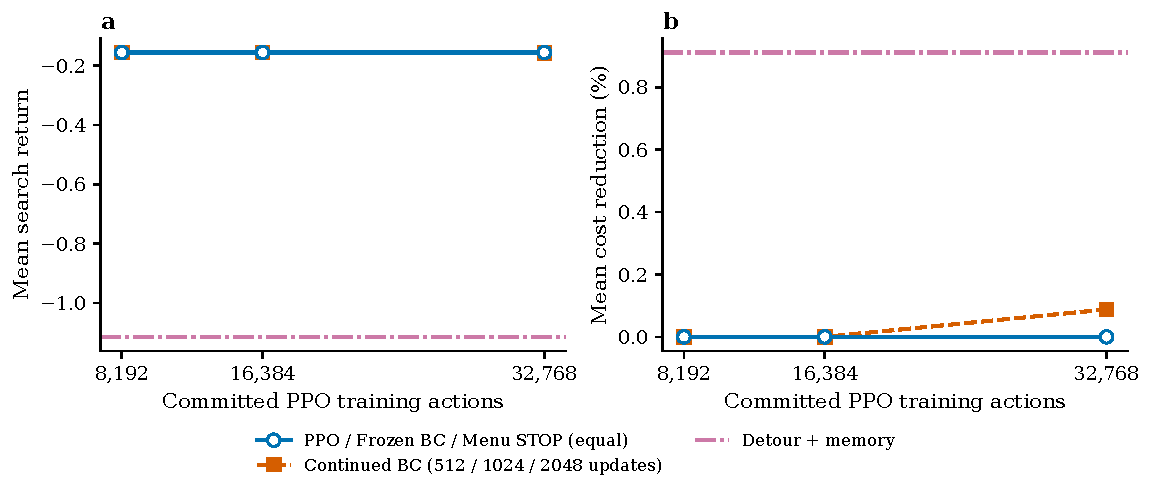
\includegraphics[width=0.96\textwidth]{figures/f1_validation.pdf}
\caption{Predeclared development checkpoints. PPO is evaluated after 8,192,
16,384 and 32,768 committed actions. The continued-BC branch uses 512, 1,024 and
2,048 additional supervised updates at the corresponding comparison points;
these are not equal-compute allocations. Each point averages the same 24
new hundred-table validation scenes. Return includes the shared work charge;
cost reduction is measured against the certified Fixed3 initial plan.
Exactly coincident PPO and constant-control series share a legend entry;
the data are not jittered.}
\label{fig:g2-validation}
\end{figure*}

\begin{figure*}[t]
\centering
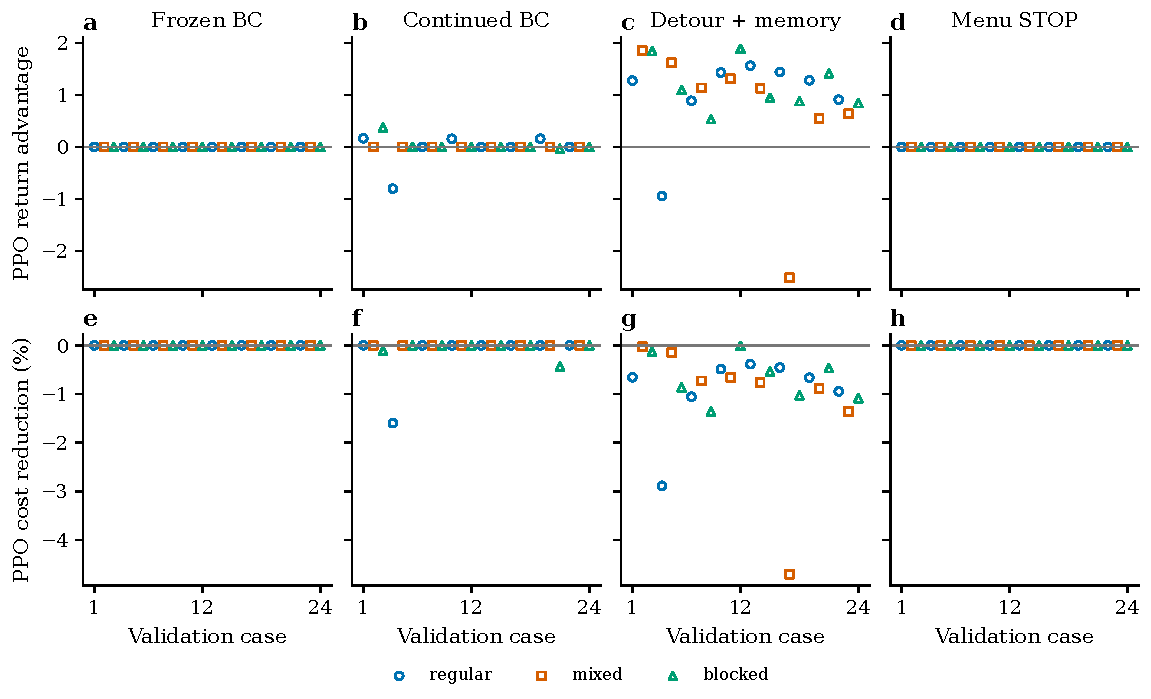
\includegraphics[width=0.96\textwidth]{figures/f2_paired.pdf}
\caption{All 24 scene-paired differences for the predeclared final PPO model.
Positive values favor PPO. Columns compare frozen BC, continued BC,
detour with shared attempt memory, and the shared-menu STOP control.
The upper row measures return difference; the lower row measures relative
cost reduction. Colors and marker shapes indicate regular, mixed and
blocked layouts. No scene or checkpoint was selected based on its result.}
\label{fig:g2-paired}
\end{figure*}

\begin{figure*}[t]
\centering
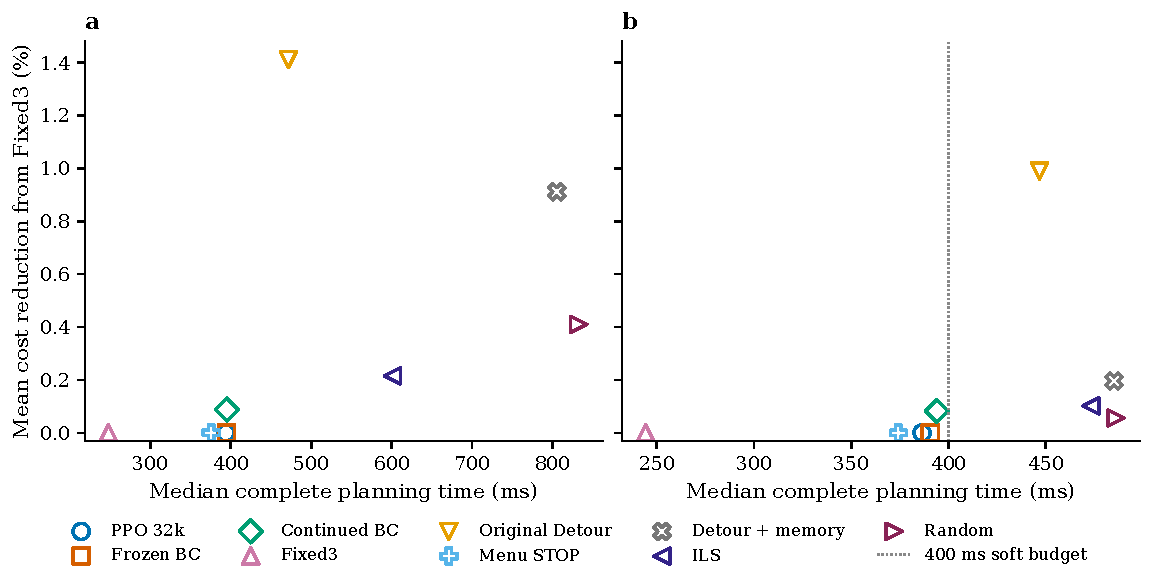
\includegraphics[width=0.96\textwidth]{figures/f3_quality_time.pdf}
\caption{Quality and full planning-time trade-off across all 24 scenes.
The horizontal coordinate is median scene-to-plan time and the vertical
coordinate is mean cost reduction from Fixed3. The left panel uses the
shared work-limited protocol; frozen original solvers are engineering
references and have no comparable G2 work reward. The right panel applies
a 400 ms complete-planning soft deadline. Preprocessing, policy decisions,
repair and final verification are included; scene generation, model loading
and output serialization are excluded. All deadline overruns are retained.}
\label{fig:g2-quality-time}
\end{figure*}

\begin{figure*}[t]
\centering
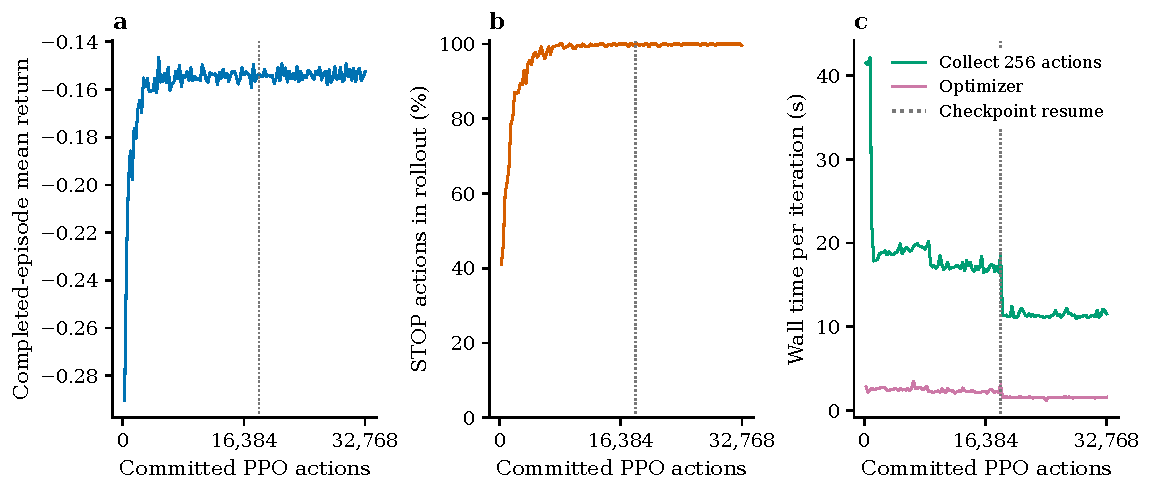
\includegraphics[width=0.96\textwidth]{figures/f4_training.pdf}
\caption{Auxiliary training diagnostics: completed-episode mean return,
STOP frequency in each 256-action rollout, and collection/optimization wall
time. These training trajectories are not deployment-quality comparisons.
Environment rollouts continue across collection boundaries; unfinished
episodes at the final action budget remain in the checkpoint. The vertical
line marks checkpoint restoration after an interrupted process; up to 256
additional uncommitted physical calls in the discarded tail cannot be counted
exactly and are not included in the horizontal axis.}
\label{fig:g2-training}
\end{figure*}
